\documentclass{standalone}
\usepackage{tikz}
\usetikzlibrary{patterns, positioning}
\usepackage[sfdefault]{ClearSans} %% option 'sfdefault' activates Clear Sans as the default text font
\usepackage[T1]{fontenc}

\begin{document}
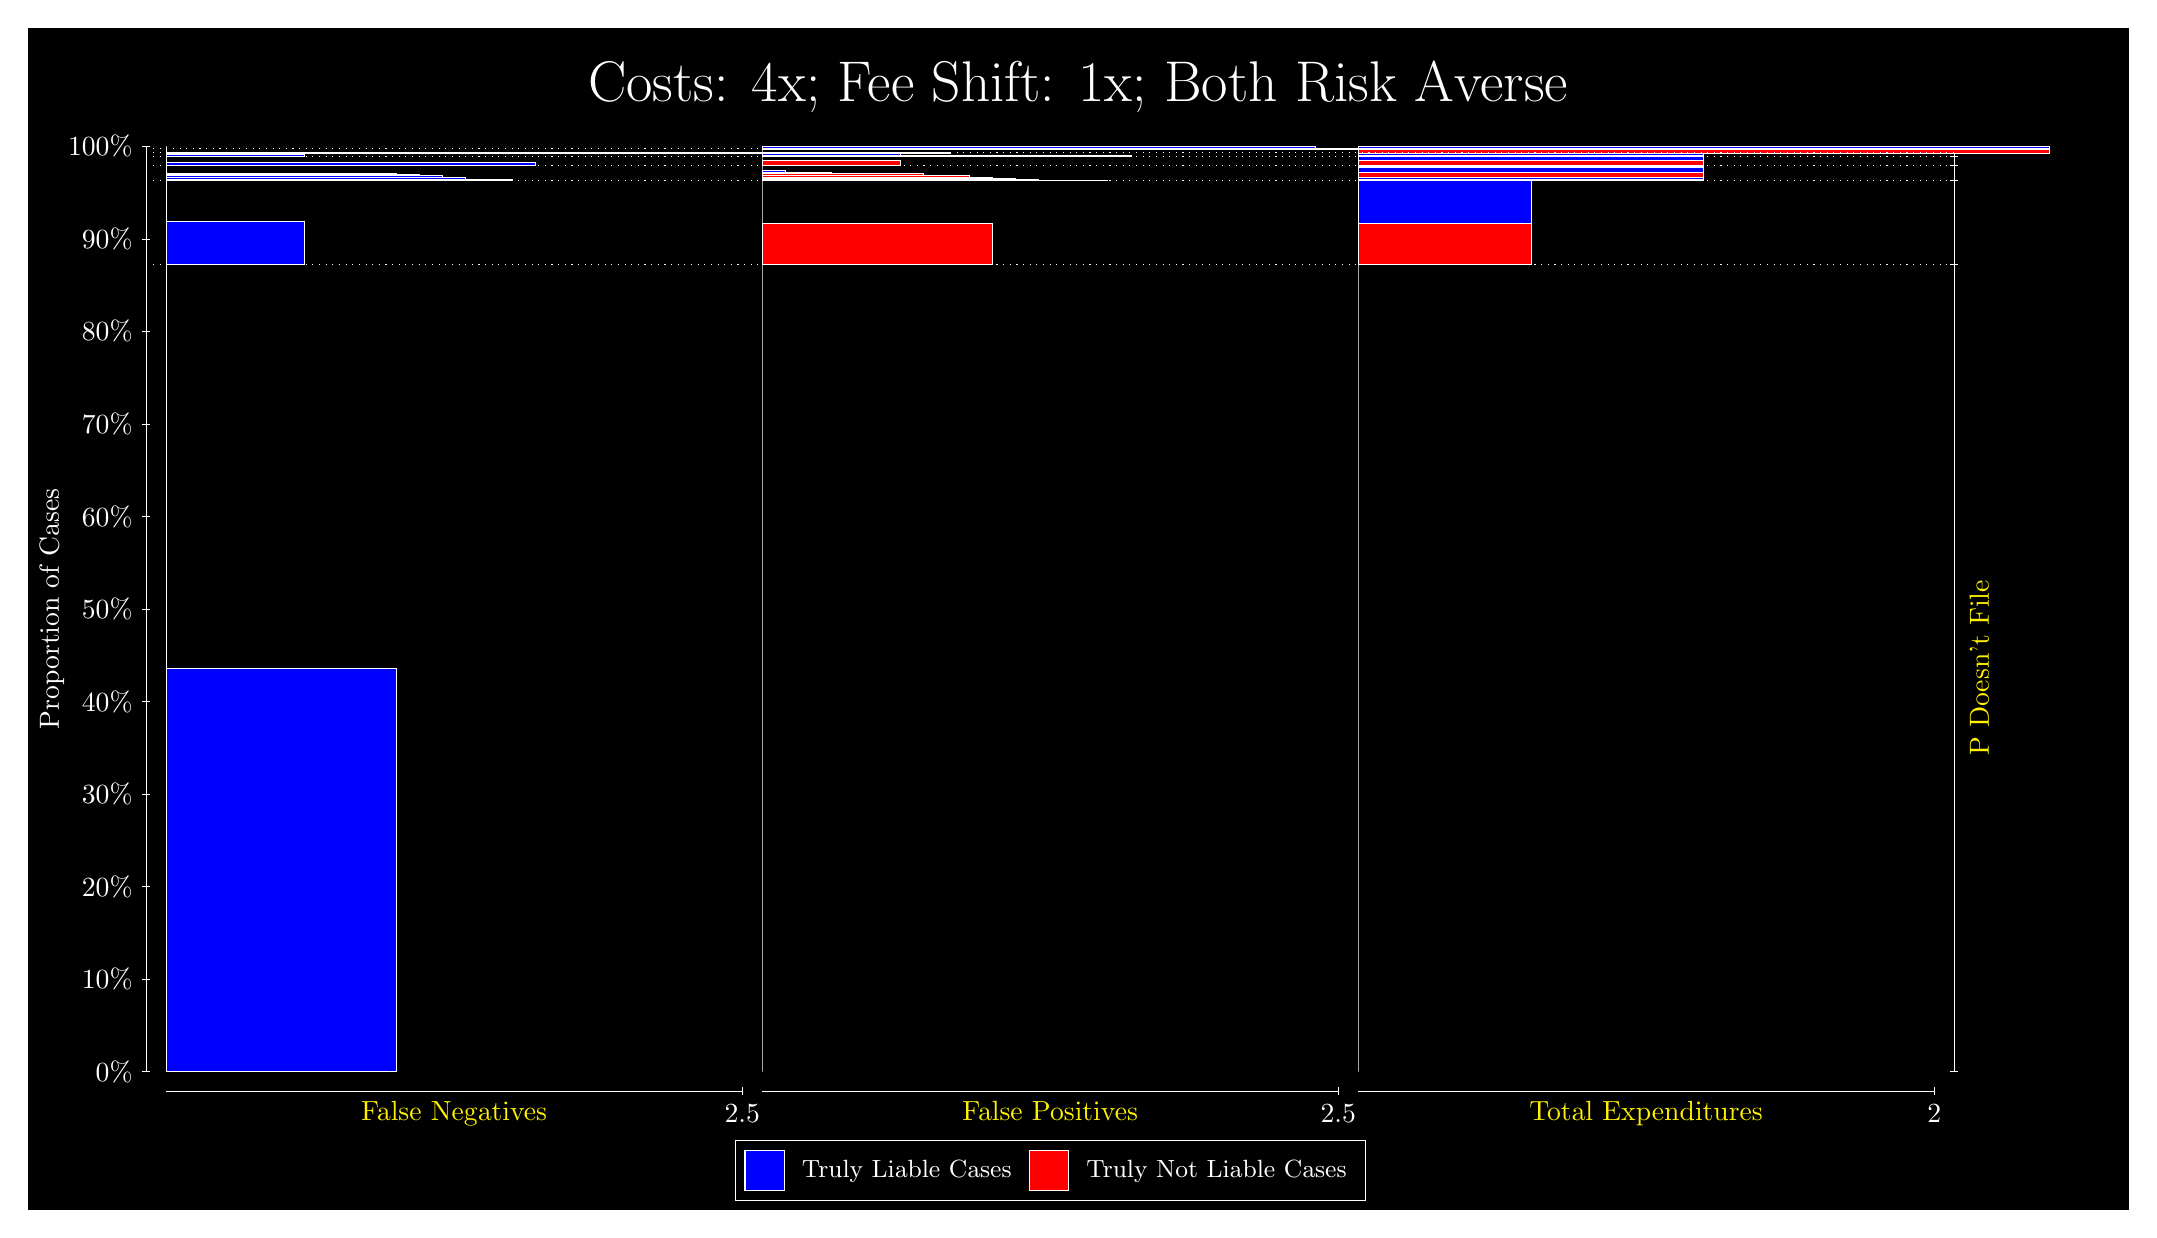
\begin{tikzpicture}
\draw[fill=black] (0,0) rectangle (26.667,15);
\draw[text=white] (0,13.5) rectangle (26.667,15) node[midway] {\huge Costs: 4x; Fee Shift: 1x; Both Risk Averse};
\draw[white, very thin] (1.5,1.75) -- (1.5,13.5);
\node[rotate=90, text=white, anchor=center] at (0.3, 7.625) {Proportion of Cases};
\draw[white, very thin] (1.45,1.75) -- (1.55,1.75);
\node[text=white, anchor=east] at (1.45, 1.75) {0\%};
\draw[white, very thin] (1.45,2.925) -- (1.55,2.925);
\node[text=white, anchor=east] at (1.45, 2.925) {10\%};
\draw[white, very thin] (1.45,4.1) -- (1.55,4.1);
\node[text=white, anchor=east] at (1.45, 4.1) {20\%};
\draw[white, very thin] (1.45,5.275) -- (1.55,5.275);
\node[text=white, anchor=east] at (1.45, 5.275) {30\%};
\draw[white, very thin] (1.45,6.45) -- (1.55,6.45);
\node[text=white, anchor=east] at (1.45, 6.45) {40\%};
\draw[white, very thin] (1.45,7.625) -- (1.55,7.625);
\node[text=white, anchor=east] at (1.45, 7.625) {50\%};
\draw[white, very thin] (1.45,8.8) -- (1.55,8.8);
\node[text=white, anchor=east] at (1.45, 8.8) {60\%};
\draw[white, very thin] (1.45,9.975) -- (1.55,9.975);
\node[text=white, anchor=east] at (1.45, 9.975) {70\%};
\draw[white, very thin] (1.45,11.15) -- (1.55,11.15);
\node[text=white, anchor=east] at (1.45, 11.15) {80\%};
\draw[white, very thin] (1.45,12.325) -- (1.55,12.325);
\node[text=white, anchor=east] at (1.45, 12.325) {90\%};
\draw[white, very thin] (1.45,13.5) -- (1.55,13.5);
\node[text=white, anchor=east] at (1.45, 13.5) {100\%};

\draw[white, very thin] (24.457,1.75) -- (24.457,13.5);
\draw[white, very thin] (24.407,1.75) -- (24.507,1.75);
\node[anchor=west] at (24.407, 1.75) {};
\draw[white, very thin] (24.407,12.002) -- (24.507,12.002);
\node[anchor=west] at (24.407, 12.002) {};
\draw[white, very thin] (24.407,13.065) -- (24.507,13.065);
\node[anchor=west] at (24.407, 13.065) {};
\draw[white, very thin] (24.407,13.253) -- (24.507,13.253);
\node[anchor=west] at (24.407, 13.253) {};
\draw[white, very thin] (24.407,13.369) -- (24.507,13.369);
\node[anchor=west] at (24.407, 13.369) {};
\draw[white, very thin] (24.407,13.416) -- (24.507,13.416);
\node[anchor=west] at (24.407, 13.416) {};
\draw[white, very thin] (24.407,13.467) -- (24.507,13.467);
\node[anchor=west] at (24.407, 13.467) {};
\draw[white, very thin] (24.407,13.5) -- (24.507,13.5);
\node[anchor=west] at (24.407, 13.5) {};

\draw[white, very thin, fill=blue] (1.75,1.75) rectangle (4.6775,6.8758);
\draw[white, very thin, fill=red] (1.75,6.8758) rectangle (1.75,12.002);
\draw[white, very thin, fill=blue] (1.75,12.002) rectangle (3.5065,12.542);
\draw[white, very thin, fill=red] (1.75,12.542) rectangle (1.75,13.065);
\draw[white, very thin, fill=blue] (1.75,13.065) rectangle (6.1413,13.078);
\draw[white, very thin, fill=blue] (1.75,13.078) rectangle (5.8486,13.084);
\draw[white, very thin, fill=blue] (1.75,13.084) rectangle (5.5558,13.106);
\draw[white, very thin, fill=blue] (1.75,13.106) rectangle (5.2631,13.126);
\draw[white, very thin, fill=blue] (1.75,13.126) rectangle (4.9703,13.147);
\draw[white, very thin, fill=blue] (1.75,13.147) rectangle (4.6775,13.153);
\draw[white, very thin, fill=blue] (1.75,13.153) rectangle (4.3848,13.159);
\draw[white, very thin, fill=blue] (1.75,13.159) rectangle (4.092,13.161);
\draw[white, very thin, fill=blue] (1.75,13.161) rectangle (3.7993,13.164);
\draw[white, very thin, fill=red] (1.75,13.164) rectangle (1.75,13.253);
\draw[white, very thin, fill=blue] (1.75,13.253) rectangle (6.4341,13.302);
\draw[white, very thin, fill=red] (1.75,13.302) rectangle (1.75,13.369);
\draw[white, very thin, fill=blue] (1.75,13.369) rectangle (3.5065,13.398);
\draw[white, very thin, fill=red] (1.75,13.398) rectangle (1.75,13.416);
\draw[white, very thin, fill=blue] (1.75,13.416) rectangle (11.704,13.424);
\draw[white, very thin, fill=red] (1.75,13.424) rectangle (1.75,13.467);
\draw[white, very thin, fill=red] (1.75,13.467) rectangle (1.75,13.474);
\draw[white, very thin, fill=blue] (1.75,13.474) rectangle (1.75,13.5);
\draw[white, very thin, fill=red] (9.3189,1.75) rectangle (9.3189,6.876);
\draw[white, very thin, fill=blue] (9.3189,6.876) rectangle (9.3189,12.002);
\draw[white, very thin, fill=red] (9.3189,12.002) rectangle (12.246,12.525);
\draw[white, very thin, fill=blue] (9.3189,12.525) rectangle (9.3189,13.065);
\draw[white, very thin, fill=red] (9.3189,13.065) rectangle (13.71,13.068);
\draw[white, very thin, fill=red] (9.3189,13.068) rectangle (13.417,13.07);
\draw[white, very thin, fill=red] (9.3189,13.07) rectangle (13.125,13.075);
\draw[white, very thin, fill=red] (9.3189,13.075) rectangle (12.832,13.081);
\draw[white, very thin, fill=red] (9.3189,13.081) rectangle (12.539,13.097);
\draw[white, very thin, fill=red] (9.3189,13.097) rectangle (12.246,13.111);
\draw[white, very thin, fill=red] (9.3189,13.111) rectangle (11.954,13.128);
\draw[white, very thin, fill=red] (9.3189,13.128) rectangle (11.661,13.134);
\draw[white, very thin, fill=red] (9.3189,13.134) rectangle (11.368,13.155);
\draw[white, very thin, fill=blue] (9.3189,13.155) rectangle (10.783,13.157);
\draw[white, very thin, fill=blue] (9.3189,13.157) rectangle (10.49,13.16);
\draw[white, very thin, fill=blue] (9.3189,13.16) rectangle (10.197,13.165);
\draw[white, very thin, fill=blue] (9.3189,13.165) rectangle (9.9044,13.171);
\draw[white, very thin, fill=blue] (9.3189,13.171) rectangle (9.6116,13.193);
\draw[white, very thin, fill=blue] (9.3189,13.193) rectangle (9.3189,13.253);
\draw[white, very thin, fill=red] (9.3189,13.253) rectangle (11.075,13.321);
\draw[white, very thin, fill=blue] (9.3189,13.321) rectangle (9.3189,13.369);
\draw[white, very thin, fill=red] (9.3189,13.369) rectangle (14.003,13.388);
\draw[white, very thin, fill=blue] (9.3189,13.388) rectangle (11.075,13.416);
\draw[white, very thin, fill=red] (9.3189,13.416) rectangle (9.3189,13.459);
\draw[white, very thin, fill=blue] (9.3189,13.459) rectangle (9.3189,13.467);
\draw[white, very thin, fill=red] (9.3189,13.467) rectangle (19.273,13.474);
\draw[white, very thin, fill=blue] (9.3189,13.474) rectangle (16.345,13.5);
\draw[white, very thin, fill=red] (16.888,1.75) rectangle (16.888,6.876);
\draw[white, very thin, fill=blue] (16.888,6.876) rectangle (16.888,12.002);
\draw[white, very thin, fill=red] (16.888,12.002) rectangle (19.083,12.525);
\draw[white, very thin, fill=blue] (16.888,12.525) rectangle (19.083,13.065);
\draw[white, very thin, fill=red] (16.888,13.065) rectangle (21.279,13.081);
\draw[white, very thin, fill=blue] (16.888,13.081) rectangle (21.279,13.102);
\draw[white, very thin, fill=red] (16.888,13.102) rectangle (21.279,13.168);
\draw[white, very thin, fill=blue] (16.888,13.168) rectangle (21.279,13.238);
\draw[white, very thin, fill=red] (16.888,13.238) rectangle (21.279,13.245);
\draw[white, very thin, fill=blue] (16.888,13.245) rectangle (21.279,13.253);
\draw[white, very thin, fill=red] (16.888,13.253) rectangle (21.279,13.321);
\draw[white, very thin, fill=blue] (16.888,13.321) rectangle (21.279,13.369);
\draw[white, very thin, fill=red] (16.888,13.369) rectangle (21.279,13.388);
\draw[white, very thin, fill=blue] (16.888,13.388) rectangle (21.279,13.416);
\draw[white, very thin, fill=red] (16.888,13.416) rectangle (25.67,13.459);
\draw[white, very thin, fill=blue] (16.888,13.459) rectangle (25.67,13.467);
\draw[white, very thin, fill=red] (16.888,13.467) rectangle (25.67,13.474);
\draw[white, very thin, fill=blue] (16.888,13.474) rectangle (25.67,13.5);
\draw[white, dotted] (1.5,12.002) -- (24.457,12.002);
\draw[white, dotted] (1.5,13.065) -- (24.457,13.065);
\draw[white, dotted] (1.5,13.253) -- (24.457,13.253);
\draw[white, dotted] (1.5,13.369) -- (24.457,13.369);
\draw[white, dotted] (1.5,13.416) -- (24.457,13.416);
\draw[white, dotted] (1.5,13.467) -- (24.457,13.467);
\draw[white, very thin] (1.75,1.5) -- (9.0689,1.5);
\node[text=yellow, anchor=north] at (5.4094, 1.5) {False Negatives};
\draw[white, very thin] (9.0689,1.45) -- (9.0689,1.55);
\node[text=white, anchor=north] at (9.0689, 1.45) {2.5};

\draw[white, very thin] (9.3189,1.5) -- (16.638,1.5);
\node[text=yellow, anchor=north] at (12.978, 1.5) {False Positives};
\draw[white, very thin] (16.638,1.45) -- (16.638,1.55);
\node[text=white, anchor=north] at (16.638, 1.45) {2.5};

\draw[white, very thin] (16.888,1.5) -- (24.207,1.5);
\node[text=yellow, anchor=north] at (20.547, 1.5) {Total Expenditures};
\draw[white, very thin] (24.207,1.45) -- (24.207,1.55);
\node[text=white, anchor=north] at (24.207, 1.45) {2};

\node[text=yellow, centered, rotate=90] at (24.777, 6.8759) {P Doesn't File};







\draw (12.978300999999998,1.5) node[draw=none] (baseCoordinate) {};
\begin{scope}[align=center]
        \matrix[scale=0.5, draw=white, below=0.5cm of baseCoordinate, nodes={draw}, column sep=0.1cm]{
            \node[rectangle, draw, minimum width=0.5cm, minimum height=0.5cm, fill=blue] {}; &
            \node[draw=none, font=\small, text=white] (B) {Truly Liable Cases}; &
            \node[rectangle, draw, minimum width=0.5cm, minimum height=0.5cm, fill=red] {}; &
            \node[draw=none, font=\small, text=white] (B) {Truly Not Liable Cases}; \\
            };
\end{scope}

\end{tikzpicture}
\end{document}